\documentclass[10pt]{article}
\usepackage[polish]{babel}
\usepackage[utf8]{inputenc}
\usepackage[T1]{fontenc}
\usepackage{amsmath}
\usepackage{amsfonts}
\usepackage{amssymb}
\usepackage[version=4]{mhchem}
\usepackage{stmaryrd}
\usepackage{graphicx}
\usepackage[export]{adjustbox}
\graphicspath{ {./images/} }

\begin{document}
\begin{enumerate}
  \item Niech \(n\) będzie liczbą naturalną. Wykaż, że suma \(1+2^{n}+3^{n}+4^{n}\) jest podzielna przez 5 wtedy i tylko wtedy, gdy \(n\) nie jest podzielne przez 4.
  \item Na szachownicy \(8 \times 8\) na kwadracie \(3 \times 3\) w jednym z naroży umieszczono 9 pionków. W jednym ruchu wybrany pionek może przemieścić się w symetrii środkowej względem dowolnego innego pionka (pod warunkiem, że docelowe pole istnieje i jest wolne). Czy można wykonać skończoną liczbę ruchów tak, by pionki ustawiły się w kwadrat \(3 \times 3\) w innym niż początkowe narożu\\
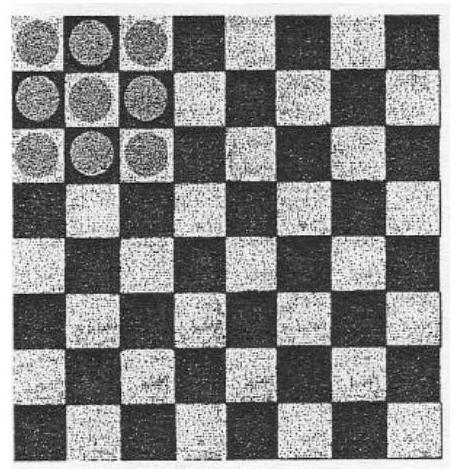
\includegraphics[max width=\textwidth, center]{2024_11_21_849b0c0f12e262df7209g-1(1)}\\
szachownicy?
  \item W trójkąt prostokątny o bokach długości \(|A B|=3,|B C|=4,|A C|=5\) wpisano dwa przystające okręgi jak na rysunku. Oblicz promienie tych okręgów.\\
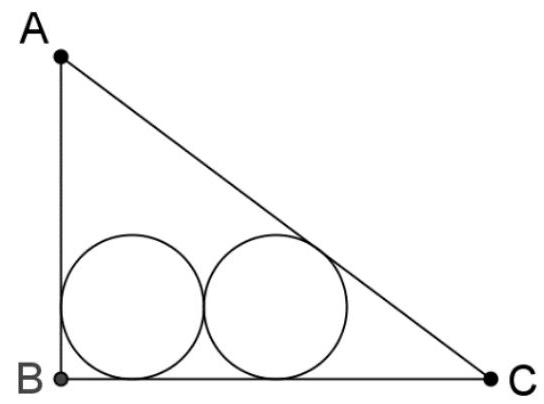
\includegraphics[max width=\textwidth, center]{2024_11_21_849b0c0f12e262df7209g-1}
\end{enumerate}

\end{document}